% Auriga theme
% find the most up-to-date version here: https://github.com/anishathalye/auriga

\documentclass[14pt,aspectratio=169]{beamer}
\usepackage{pgfpages}
\usepackage{fancyvrb}
\usepackage{tikz}
\usepackage{pgfplots}
\usepackage{booktabs}
\usepackage{pgffor}
\pgfplotsset{compat=1.18}

% Define colors
\definecolor{c1}{HTML}{CB6040}
\definecolor{c2}{HTML}{A66E38}
\definecolor{c3}{HTML}{FD8B51}
\definecolor{c4}{HTML}{257180}
% Use natbib with author-year citation style
%\usepackage[authoryear]{natbib}

% Add the bibliography style compatible with author-year
%\bibliographystyle{plainnat}
\definecolor{red}{RGB}{181, 23, 0}
\definecolor{blue}{RGB}{0, 118, 186}
\definecolor{gray}{RGB}{50, 50, 50}

\newcommand{\cx}{\textcolor{c1}{x}}
\newcommand{\cy}{\textcolor{c3}{y}}
\newcommand{\cz}{\textcolor{c4}{z}}

\newcommand{\Ver}{\textcolor{c2}{\text{Ver}}}

\newcommand{\cfy}[1]{\textcolor{c3}{#1}}
\newcommand{\cfr}[1]{\textcolor{c2}{#1}}
\newcommand{\cfz}[1]{\textcolor{c4}{#1}}
\newcommand{\czT}{\cfz{z_{1:T}}}

\setbeamercolor{palette primary}{fg=c1,bg=white}
\setbeamercolor{palette secondary}{fg=c2,bg=white}
\setbeamercolor{palette tertiary}{bg=c3,fg=white}
\setbeamercolor{palette quaternary}{fg=black,bg=white}
\setbeamercolor{structure}{fg=c1}


\setbeamertemplate{bibliography item}[text]

\renewcommand{\footnote}[1]{
    \begin{tikzpicture}[remember picture,overlay]
        \node[anchor=north east, xshift=-0.2cm, yshift=-0.2cm] at (current page.north east) {\footnotesize #1};
    \end{tikzpicture}
}
\usepackage{tcolorbox}
\usetheme{auriga}
\usecolortheme{auriga}
\setbeamercolor{math text}{fg=gray}

\newcommand\blfootnote[1]{%
\begingroup
\renewcommand\thefootnote{}\footnote{\hfill\parbox[t]{0.5\textwidth}{\raggedleft #1}}%
\addtocounter{footnote}{-1}%
\endgroup
}

%\setbeamertemplate{footline}[]
%\renewcommand\footnotemark{}

% define some colors for a consistent theme across slides
\title{Speculations \\ on \\ Test-Time Scaling}
\author{Sasha Rush \  Daniel Ritter}

\institute[shortinst]{Cornell}
% \institute[shortinst]{\inst{*} Preprint}

\setcounter{tocdepth}{1}
\begin{document}

\frame{\titlepage}


\section{Introduction}

\begin{frame}[t]{}
	\vspace{1cm}
	\begin{center}
		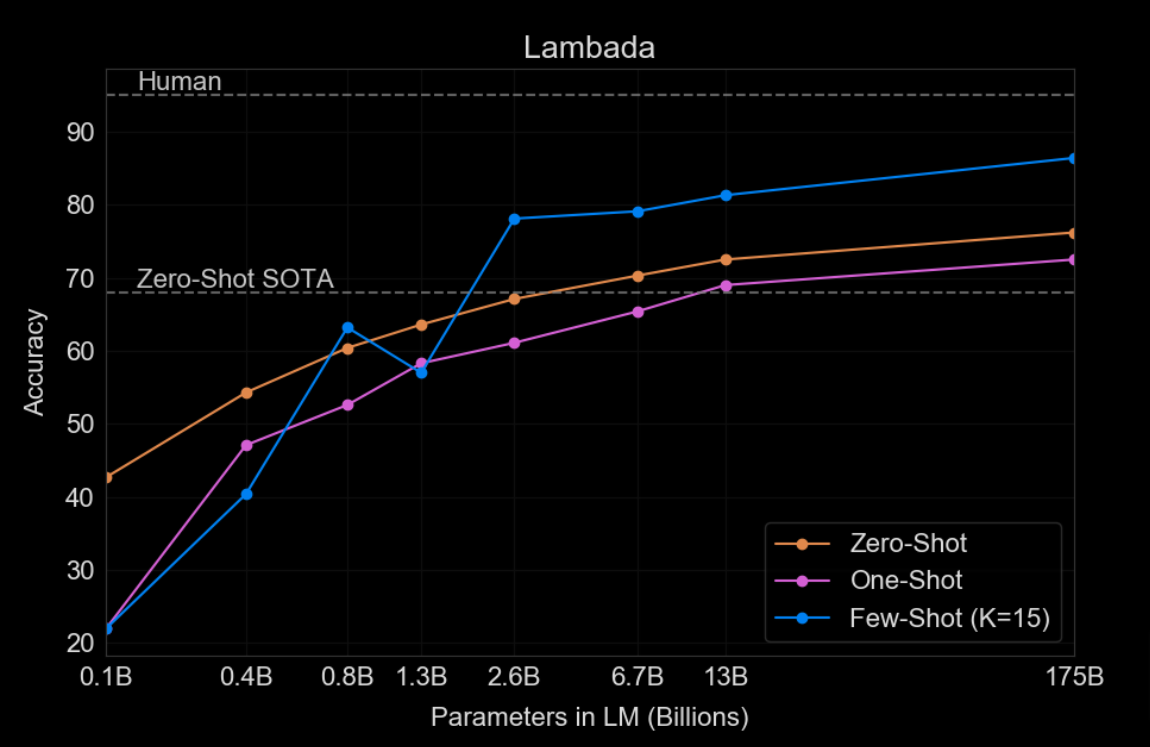
\includegraphics[width=0.8\linewidth]{images/gpt3i}
	\end{center}
	\note{
		LLM (2018-2024) driven by training scaling
		Speculation: Benefit of static data running out
		o1 - Large-scale RL Training leading to search usage.
	}
	\blfootnote{\cite{Brown2020-on}}
\end{frame}


\begin{frame}[t]{}
	\vspace{1cm}
	\begin{center}
		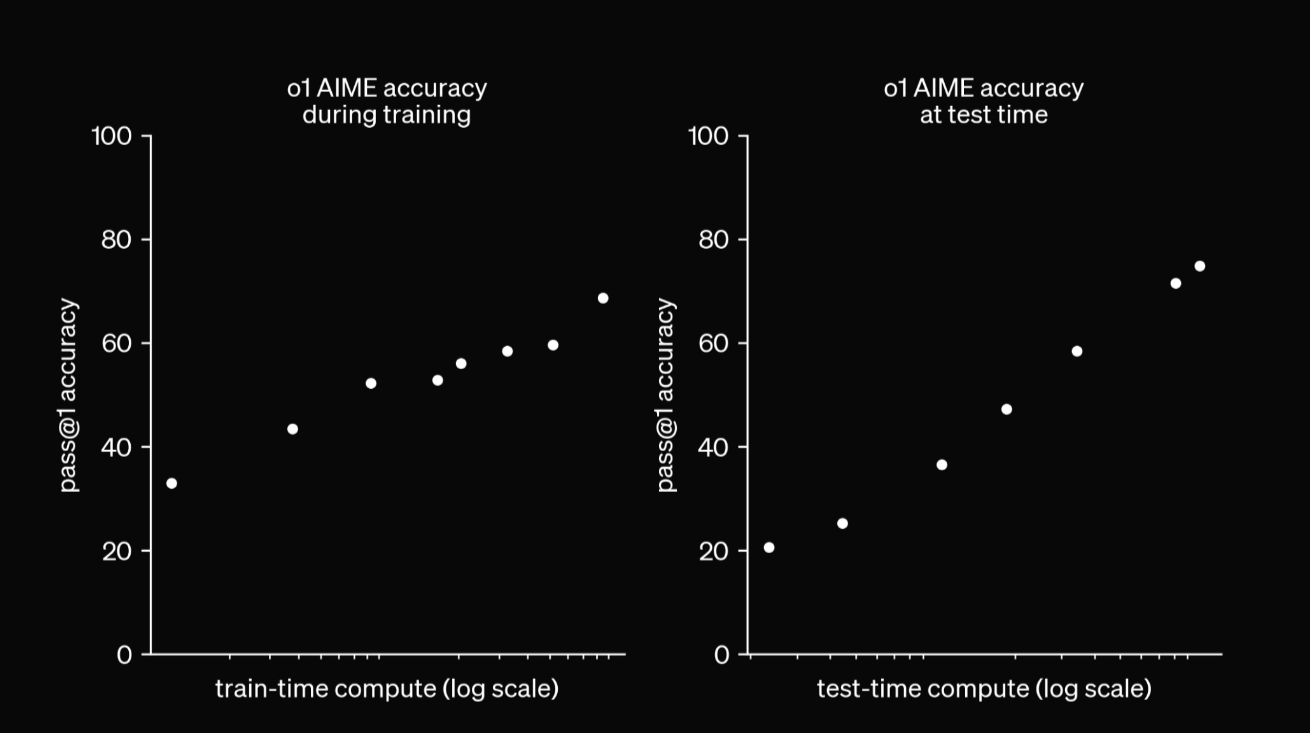
\includegraphics[width=0.8\linewidth]{images/compute.png}
	\end{center}
	\blfootnote{\cite{OpenAIUnknown-zp}}
\end{frame}

\begin{frame}{AIME}
	\begin{tcolorbox}[colback=white,colframe=black,boxrule=0.5pt]
		\small
		For any finite set $X$, let $| X |$ denote the number of elements in $X$. Define \[S_n = \sum | A \cap B | ,\] where the sum is taken over all ordered pairs $(A, B)$ such that $A$ and $B$ are subsets of $\left\{ 1 , 2 , 3, \cdots , n \right\}$ with $|A| = |B|$. For example, $S_2 = 4$ because the sum is taken over the pairs of subsets \[(A, B) \in \left\{ (\emptyset, \emptyset) , ( \{1\} , \{1\} ), ( \{1\} , \{2\} ) , ( \{2\} , \{1\} ) , ( \{2\} , \{2\} ) , ( \{1 , 2\} , \{1 , 2\} ) \right\}\] giving $S_2 = 0 + 1 + 0 + 0 + 1 + 2 = 4$. Let $\frac{S_{2022}}{S_{2021}} = \frac{p}{q}$, where $p$ and $q$ are relatively prime positive integers. Find the remainder when $p + q$ is divided by 1000.
	\end{tcolorbox}
	\blfootnote{\cite{Hendrycks2021-jr}}
\end{frame}

\begin{frame}{The Bitter Lesson}
	\begin{columns}
		\begin{column}{0.3\textwidth}
			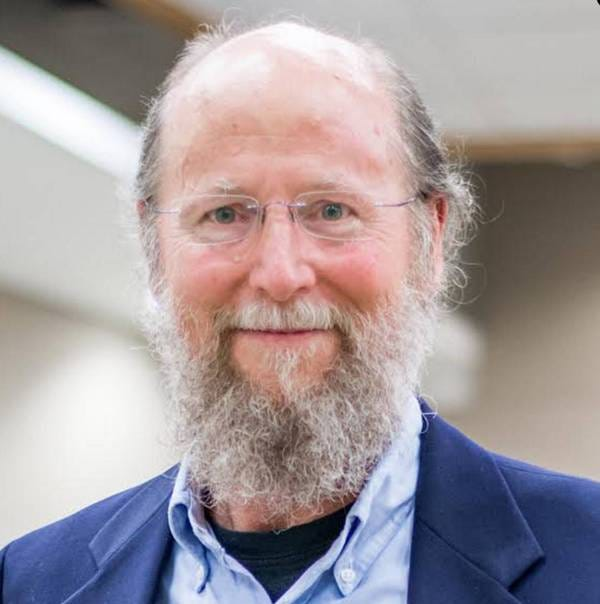
\includegraphics[width=\linewidth]{images/Sutton}
		\end{column}
		\begin{column}{0.7\textwidth}
			\begin{tcolorbox}[colback=white,colframe=black,boxrule=0.5pt]
				The bitter lesson is based on the historical observations that 1) AI researchers have often tried to build knowledge into their agents,
				2) this always helps in the short term, and is personally satisfying to the researcher, but 3) in the long run it plateaus and even inhibits
				further progress, and 4) breakthrough progress eventually arrives by an opposing approach based on scaling computation by \textbf{search and learning}.
			\end{tcolorbox}
		\end{column}
	\end{columns}

	\blfootnote{\cite{Sutton2019-my}}
\end{frame}


\begin{frame}{Importance of Search}
	\begin{columns}
		\begin{column}{0.3\textwidth}
			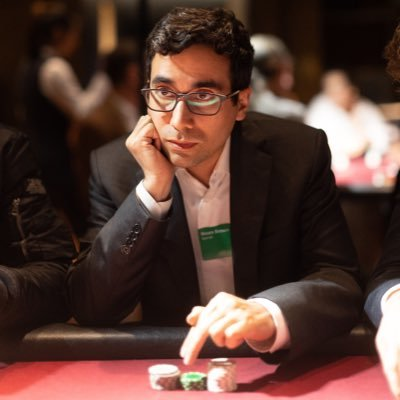
\includegraphics[width=\linewidth]{images/Noam}
		\end{column}
		\begin{column}{0.7\textwidth}
			\begin{tcolorbox}[colback=white,colframe=black,boxrule=0.5pt]
				The most important [lesson] is that I and other researchers simply didn't know how much of a difference scaling up search would make.
				If I had seen those scaling results at the start of my PhD, I would have shifted to researching search algorithms for poker much sooner
				and we probably would have gotten superhuman poker bots much sooner.
			\end{tcolorbox}
		\end{column}
	\end{columns}
	\blfootnote{\cite{Brown2017-of},\url{https://x.com/polynoamial/status/1840822629625688469}}
\end{frame}


\begin{frame}{Sources}
	\begin{itemize}
		\item Survey of the public literature
		\item Synthesis of discussions with expert
		\item Rumors from social media
	\end{itemize}

	\vspace{1cm}

	\begin{small}
		Thanks to Lewis Tunstall, Edward Beeching, Aviral Kumar, Charlie Snell,
		Michael Hassid, Yoav Artzi, Risab Agarwal, Kanishk Gandhi,
		Wenting Zhao, Yuntian Deng, Nathan Lambert, Noah Goodman
	\end{small}
\end{frame}

\section{The Clues}

\begin{frame}{Outline}
	\tableofcontents[hideallsubsections, currentsection]
\end{frame}

\begin{frame}{o1 Description}
	\begin{columns}
		\begin{column}{0.3\textwidth}
			
\includegraphics[width=\linewidth]{images/openai}
		\end{column}
		\begin{column}{0.7\textwidth}
			\begin{tcolorbox}[colback=white,colframe=black,boxrule=0.5pt]
				Our large-scale \textbf{reinforcement learning algorithm} teaches the model
				how to think productively using its \textbf{chain of thought} in a highly
				\textbf{data-efficient} training process.
			\end{tcolorbox}
		\end{column}
	\end{columns}
	\blfootnote{\cite{OpenAIUnknown-zp}}
\end{frame}

\begin{frame}{Implication}
	\begin{itemize}
		\item \structure{RL}; Signal from verifiable problems
		\item \structure{CoT}; Test-time occurs in token stream
		\item \structure{Data-Efficient}; Bounded set of problems
	\end{itemize}
\end{frame}

\begin{frame}{Current Assumptions}
	\begin{itemize}
		\item Single final language model
		\item Not following from expert examples
		\item Behaviors are learned
	\end{itemize}
\end{frame}

\begin{frame}{Review: Chain of Thought}
	\begin{columns}
		\begin{column}{0.4\linewidth}
			\begin{itemize}
				\item The model generates intermediate steps.
				\item These steps provide an scratchpad for technical problems.
			\end{itemize}
		\end{column}
		\begin{column}{0.6\linewidth}
			\begin{tcolorbox}[colback=white,colframe=black,boxrule=0.5pt]

				\begin{small}
					\textcolor{c1}{Question: 4 baskets. 3 have 9 apples, 15 oranges, 14 bananas each. 4th has 2 less of each. Total fruits?}

					\textcolor{c4}{Let's solve step-by-step:}

					\textcolor{c4}{Fruits in one of first 3 baskets: 9 + 15 + 14 = 38}

					\textcolor{c4}{Total in first 3 baskets: 38 * 3 = 114}

					\textcolor{c4}{4th basket: (9-2) + (15-2) + (14-2) = 32}

					\textcolor{c4}{Total fruits: 114 + 32 = 146}

					\textcolor{c3}{Answer: 146 fruits}
				\end{small}
			\end{tcolorbox}
		\end{column}

	\end{columns}
	\blfootnote{\cite{Wei2022-uj,Nye2021-bx}}
\end{frame}

\begin{frame}{o1 Chain of Thought}
	\begin{columns}
		\begin{column}{0.3\textwidth}
			
\includegraphics[width=\linewidth]{images/openai}
		\end{column}
		\begin{column}{0.7\textwidth}
			\begin{tcolorbox}[colback=white,colframe=black,boxrule=0.5pt]
				o1 learns to hone its chain of thought and refine the strategies it uses.
				It learns to recognize and \textbf{correct its mistakes}.
				It learns to \textbf{break down tricky steps} into simpler ones.
				It learns to try a \textbf{different approach} when the current one isn't working.
			\end{tcolorbox}
		\end{column}
	\end{columns}
	\blfootnote{\cite{OpenAIUnknown-zp}}
\end{frame}

\begin{frame}{o1 CoT: Outlining}
	\begin{tcolorbox}[colback=white,colframe=black,boxrule=0.5pt]
		\begin{quote}
			Implementation Outline:

			1. Capture input string as argument.

			2. Remove any spaces (if any).

			3. Parse input string to extract numbers as arrays.

			- Since the input is in the format '[1,2],[3,4]', we can:

			- Remove outer brackets if necessary.

			- Split the string by '],' to get each row.

			- For each row, remove '[' and ']', then split by ',' to get elements.


			4. Build a 2D array in bash (arrays containing arrays).
		\end{quote}
	\end{tcolorbox}
	\blfootnote{\cite{OpenAIUnknown-zp}}
\end{frame}


\begin{frame}{o1 CoT: Planning}
	\begin{tcolorbox}[colback=white,colframe=black,boxrule=0.5pt]
		\begin{quote}
			First, the cipher seems connected to the plaintext.
			\vspace{0.3cm}

			Given the time constraints, perhaps the easiest way is to try to see patterns.
			\vspace{0.3cm}

			Option 1: Try to find mapping from letters to letters.
			\vspace{0.3cm}

			Do any letters match?
			\vspace{0.3cm}

			First, let's write down the ciphertext and plaintext letters on top of each other.
		\end{quote}
	\end{tcolorbox}
	\blfootnote{\cite{OpenAIUnknown-zp}}
\end{frame}

\begin{frame}{o1 CoT: Backtracking}
	\begin{tcolorbox}[colback=white,colframe=black,boxrule=0.5pt]
		\begin{quote}
			Similarly, m(x)* (−x 2) = (−x2n + 2 + m2n−2x2n + lower terms)m(x) * (−x 2) = (−x 2n + 2 + m 2n−2 x 2n + lower terms).

			\vspace{0.3cm}
			Wait, actually, this may not help us directly without specific terms.An alternative is to consider the known polynomials.

			\vspace{0.3cm}

			So m(x) = k ...
		\end{quote}
	\end{tcolorbox}
	\blfootnote{\cite{OpenAIUnknown-zp}}
\end{frame}

\begin{frame}{o1 CoT: Self-Evaluation}

	\begin{tcolorbox}[colback=white,colframe=black,boxrule=0.5pt]
		\begin{quote}

			Let’s analyze each option.
			\vspace{0.3cm}

			Option A: “because appetite regulation is a field of staggering complexity.”
			\vspace{0.3cm}

			Is that a good explanation? Hmm.
			\vspace{0.3cm}

			Option B: “because researchers seldom ask the right questions.”
			\vspace{0.3cm}

			Does this make sense with the main clause?
		\end{quote}
	\end{tcolorbox}
	\blfootnote{\cite{OpenAIUnknown-zp}}
\end{frame}

\begin{frame}{Summary}
	\begin{itemize}
		\item CoT provides test-time scaling
		\item CoT looks like search / planning in a classical sense
		\item RL needed to induce this behavior
	\end{itemize}
\end{frame}

\section{Technical Background}

\begin{frame}{Outline}
	\tableofcontents[hideallsubsections, currentsection]
\end{frame}

\begin{frame}{Technical Background}
	\begin{columns}
		\begin{column}{0.4\linewidth}
			\begin{itemize}
				\item Formalize sampling of latent reasoning
				\item Techniques from combinatorial sampling
				\item No learning yet.
			\end{itemize}
		\end{column}
		\begin{column}{0.6\linewidth}
			\begin{tcolorbox}[colback=white,colframe=black,boxrule=0.5pt]

				\begin{small}
					\textcolor{c1}{Question: 4 baskets. 3 have 9 apples, 15 oranges, 14 bananas each. 4th has 2 less of each. Total fruits?}

					\textcolor{c4}{Let's solve step-by-step:}

					\textcolor{c4}{Fruits in one of first 3 baskets: 9 + 15 + 14 = 38}

					\textcolor{c4}{Total in first 3 baskets: 38 * 3 = 114}

					\textcolor{c4}{4th basket: (9-2) + (15-2) + (14-2) = 32}

					\textcolor{c4}{Total fruits: 114 + 32 = 146}

					\textcolor{c3}{Answer: 146 fruits}
				\end{small}
			\end{tcolorbox}
		\end{column}
	\end{columns}
	\blfootnote{\cite{Cobbe2021-gt}}
\end{frame}


\begin{frame}{Stepwise CoT Sampling}
	\begin{itemize}
		\item $\cx$;  problem specification
		\item $\cfz{z_{1:T}} \in {\mathcal{S}^T}$; chain of thought (CoT) steps
		\item $\cy \in \cfy{\mathcal Y}$; final answer
		      $$p(\cy | \cx) = \mathbb{E}_{\cz} p(\cy|\cx,\cz)$$
	\end{itemize}
	\blfootnote{\cite{Welleck2024-yr}}
\end{frame}

\begin{frame}{Warm-up: Ancestral Sampling}
	\begin{columns}
		\begin{column}{0.5\linewidth}
			\begin{align*}
				{\czT} & \sim p(\cdot | \cx)         \\
				{\cy}  & \sim p(\cdot | \cx, {\czT})
			\end{align*}
		\end{column}
		\begin{column}{0.5\linewidth}
			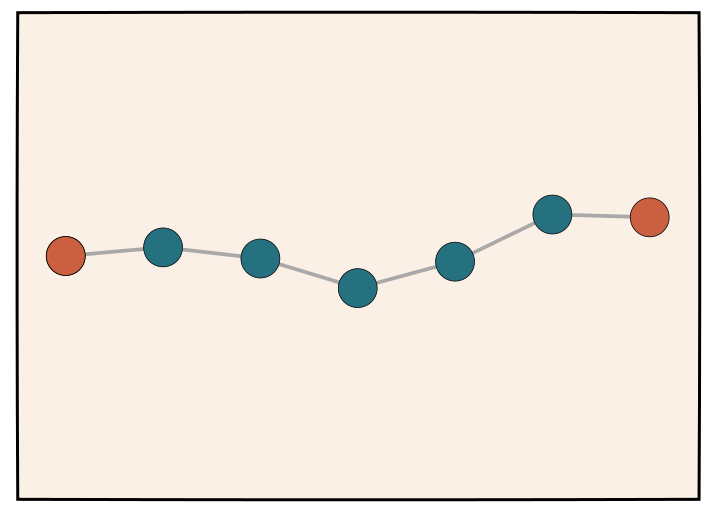
\includegraphics[width=\textwidth]{images/ancestral.png}
		\end{column}
	\end{columns}
	\vspace{1cm}
	$T$ is the amount of test-time compute
	\blfootnote{\cite{Wei2022-uj}}
\end{frame}

\begin{frame}{Monte-Carlo Self-Consistency}
	\begin{columns}
		\begin{column}{0.5\linewidth}
			For $N$ samples,
			\begin{align*}
				{\czT} & \sim p(\cdot | \cx)         \\
				\cy^n  & \sim p(\cdot | \cx, {\czT})
			\end{align*}
			\vspace{1cm}
			Pick majority choice $\cy^n$
		\end{column}
		\begin{column}{0.5\linewidth}
			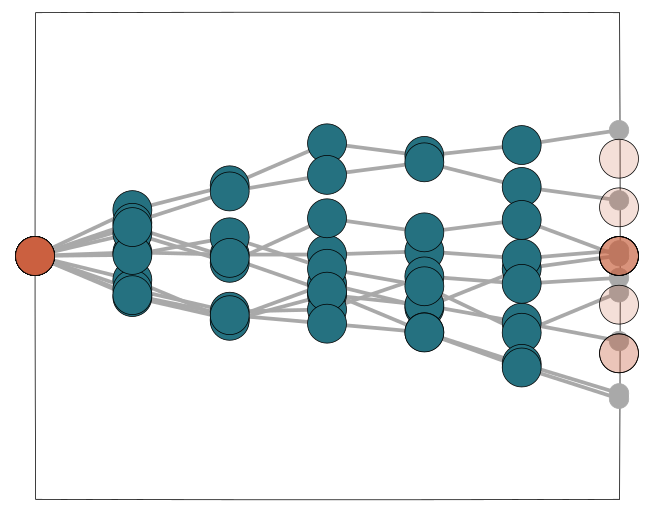
\includegraphics[width=\textwidth]{images/bwalk.png}
		\end{column}
	\end{columns}
	\blfootnote{\cite{Wang2022-px}}
\end{frame}

\begin{frame}{Assumption: Verifier}
	$$\text{Ver}_x : \cfy{\mathcal{Y}} \rightarrow \{0, 1\}$$

	Common datasets:
	\begin{itemize}
		\item Regular expression for math \cite{Cobbe2021-gt}
		\item Unit test for code \cite{Hendrycks2021-nv}
		\item Test qukestions for science \cite{Hendrycks2021-tt}
	\end{itemize}
	\blfootnote{\cite{Uesato2022-aw}}
\end{frame}


\begin{frame}{Rejection Sampling \\ Best-of-N}
	\begin{columns}
		\begin{column}{0.5\linewidth}
			For $n = 1$ to $N$:
			\begin{align*}
				\cz^n & \sim p(\cz | \cx)        \\
				\cy^n & \sim p(\cy | \cx, \cz^n)
			\end{align*}
			Verified set $\{\cy^n : \Ver_x(\cy^n) \}$
		\end{column}
		\begin{column}{0.5\linewidth}
			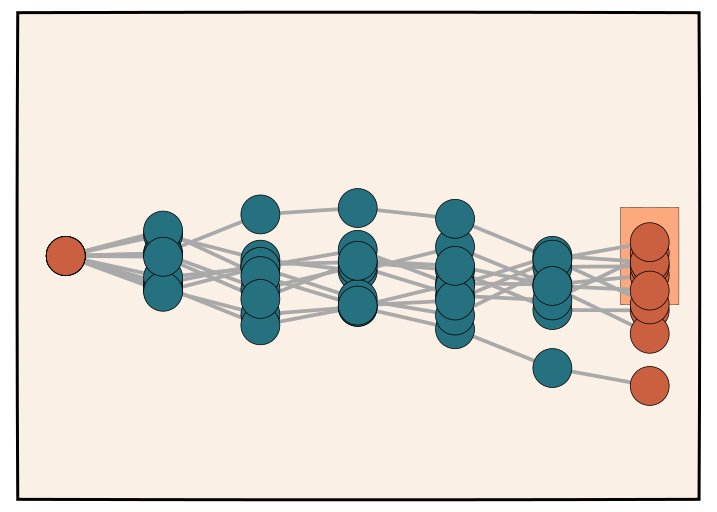
\includegraphics[height=0.3\textheight]{images/rejecta.png}
			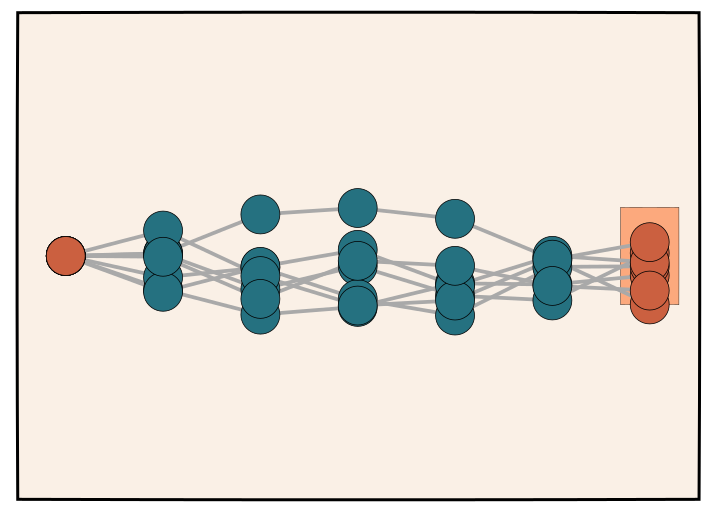
\includegraphics[height=0.3\textheight]{images/rejectb.png}
		\end{column}
	\end{columns}
	\blfootnote{\cite{Nakano2021-iz,Lightman2023-cr}}
\end{frame}


\begin{frame}{Monte-Carlo Roll-Outs}
	\begin{columns}
		\begin{column}{0.5\linewidth}
			Given partial CoT $\cfz{z_{1:t}}$, expected value,

			$$\mathbb{E}_{\cy\sim p(\cdot| \cx)}\  \Ver(\cy)$$

			Monte Carlo for this expectation.
		\end{column}
		\begin{column}{0.5\linewidth}
			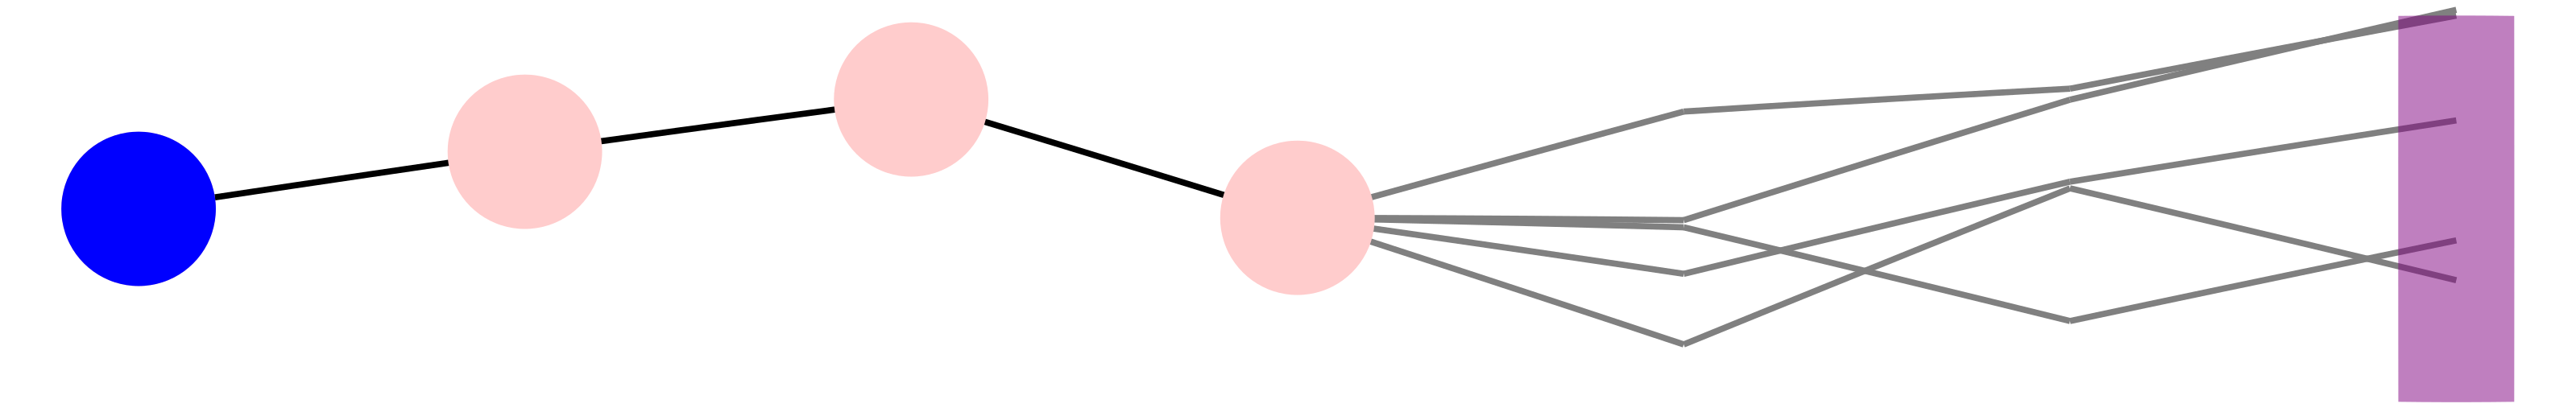
\includegraphics[width=\textwidth]{images/mcroll.png}
		\end{column}
	\end{columns}
	\blfootnote{\cite{Wang2023-ur}}
\end{frame}



\begin{frame}{Goal: Learning with Latent CoTs}
	\begin{columns}
		\begin{column}{0.5\linewidth}
			Maximum likelihood;

			\begin{align*}
				\max_{\theta} & \sum \log p(\cy | \cx; \theta)  =                    \\
				              & \sum \log \mathbb{E}_{\cz} p(\cy | \cx, \cz; \theta)
			\end{align*}

			Classic combinatorial expectation
		\end{column}
		\begin{column}{0.5\linewidth}
			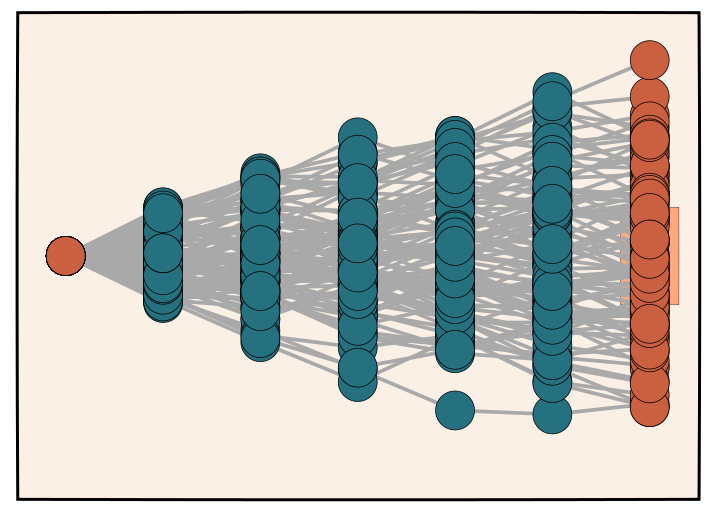
\includegraphics[width=\textwidth]{images/all.png}
		\end{column}
	\end{columns}
\end{frame}

\section{The Suspects}

\begin{frame}{Outline}
	\tableofcontents[hideallsubsections, currentsection]
\end{frame}

\begin{frame}{The Suspects}
	\begin{itemize}
		\item Guess + Check
		\item Guided Search
		\item AlphaZero
		\item Learning to Correct
	\end{itemize}
\end{frame}

\begin{frame}{The Suspects}
	\begin{itemize}
		\item \structure{Guess + Check}
		\item Guided Search
		\item AlphaZero
		\item Learning to Correct
	\end{itemize}
\end{frame}

\subsection{Guess + Check}

\begin{frame}{Suspect 1: Guess + Check}
	\begin{columns}
		\begin{column}{0.5\linewidth}
			\begin{itemize}
				\item 1) Sample $N$ CoTs
				\item 2) Check if successful
				\item 3) Train on good ones
			\end{itemize}
		\end{column}
		\begin{column}{0.5\linewidth}
			\begin{center}
				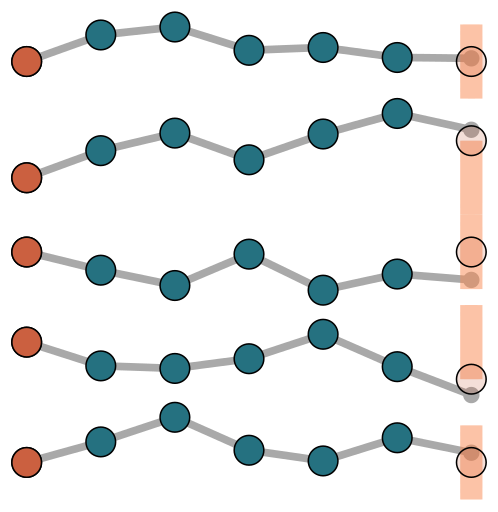
\includegraphics[height=0.8\textheight]{images/reject1}
			\end{center}
		\end{column}
	\end{columns}
\end{frame}

\begin{frame}{Framework: Rejection Sampling EM}
	$$\max_{\theta} \sum \log E_{\cz \sim p({\cz} | \cx;\theta)} p(\cy|  \cx, \cz)$$
	\begin{itemize}
		\item E-Step: For $n = 1$ to $N$:
		      \begin{align*}
			      \cz^n & \sim p(\cdot | \cx)        \\
			      \cy^n & \sim p(\cdot | \cx, \cz^n)
		      \end{align*}
		      Keep verified set $\mathcal{Z} = \{\cz^n : \Ver(\cy^n)\}$
		\item M-Step: Fit $\theta' \gets \arg\max_{\theta}
			      \sum_{{\cz} \in \mathcal{Z}} \log p({\cz} | \cx;\theta)$
	\end{itemize}
	\blfootnote{\cite{Neal1998-np}}
\end{frame}



\begin{frame}{Variants}
	\begin{itemize}
		\item Best-of-N Training \cite{Cobbe2021-gt}
		\item STaR \cite{Zelikman2022-id}
		\item ReST \cite{Gulcehre2023-vk}
		\item ReST-EM \cite{Singh2023-eb}
		\item Filtered Rejection Sampling \cite{Nakano2021-iz}
	\end{itemize}
\end{frame}


\begin{frame}{Reinforcement Learning?}
	\begin{itemize}
		\item Batched $\rightarrow$ Compute trajectories first, then train
		\item Online $\rightarrow$  Update after each example
		\item Specific algorithm choice (PPO, etc)
	\end{itemize}
\end{frame}



\begin{frame}{Empirical Results}
	% None of STaR, ReST, ReST-EM compare directly to self-consistency alone.
	% The closest is ReST-EM, which says that using a self-consistency on
	% the Rest-EM model gets better performance than using it on the base model (but without a figure).
	% I'm putting in figure 5 from Rest-EM for now, which shows that sampling produces
	% a correct answer more often from Rest-EM than from the base model across a range of sample
	% sizes. It doesn't show how far below these two lines self-consistency would be, but it's at least
	% evidence that Rest-EM improves on the base model. And the Pass@K performance should upper bound
	% the performance of self-consistency, since anything correct under majority voting is also correct
	% in Pass@K.
	\blfootnote{\cite{Singh2023-eb}}
	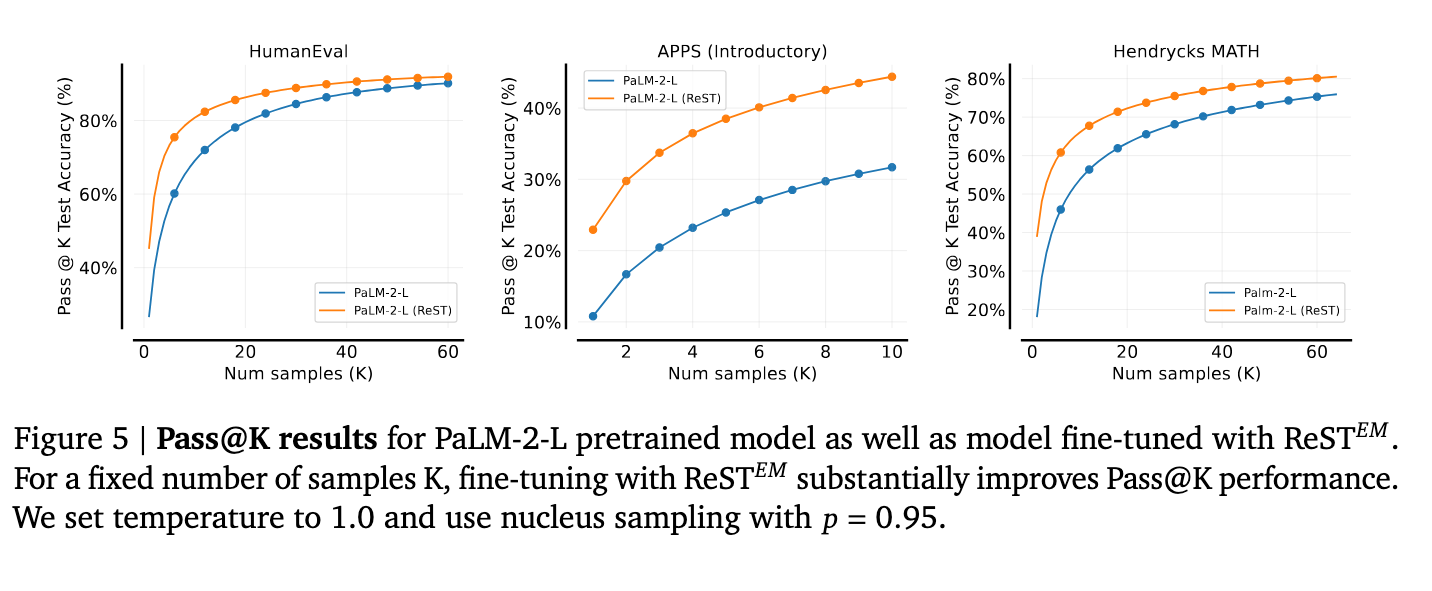
\includegraphics[width=\textwidth]{images/rest_em_figure_5.png}
\end{frame}



\begin{frame}{Is this o1?}
	\begin{columns}
		\begin{column}{0.5\linewidth}
			\textbf{Pro}
			\vspace{0.3cm}
			\begin{itemize}
				\item[$\boldsymbol{\checkmark}$] Extremely simple and scalable
				\item[$\boldsymbol{\checkmark}$] Positive results in past work

			\end{itemize}
		\end{column}
		\begin{column}{0.5\linewidth}
			\pause
			\begin{itemize}
				\item[\textcolor{red}{$\boldsymbol{\times}$}] No evidence this learns to correct, plan
				\item[\textcolor{red}{$\boldsymbol{\times}$}] Computationally inefficient search
			\end{itemize}
		\end{column}
	\end{columns}
\end{frame}

\subsection{Guided Search}

\begin{frame}{The Suspects}
	\begin{itemize}
		\item Guess + Check
		\item \structure{Guided Search}
		\item AlphaZero
		\item Learning to Correct
	\end{itemize}
\end{frame}


\begin{frame}{Suspect 2: Guided Search}
	\begin{itemize}
		\item 1) During CoT sampling, use a heuristic to
		      improve trajectories
		\item 2) Check if final versions are successful
		\item 3) Train on good ones
	\end{itemize}
\end{frame}


\begin{frame}{Framework: Beam Search with Guide}
	% Slightly different from token level beam search since we can't enumerate all the possible z_t like in a vocabulary,
	% so instead sample an initial k of them, score those with r and keep the top m
	%
	% A bit light on notation here (e.g. didn't define the set of z_t for each candidate prefix explicitly) to
	% avoid a lot of indices, but can add that if it needs to be more formal.
	\begin{columns}
		\begin{column}{0.5\linewidth}
			$\cfr{r}: \cfz{\mathcal{S}^t} \rightarrow \mathbb{R}$; Guide function
			\vspace{0.3cm}
			\pause

			For each step $t$,
			\begin{enumerate}
				\item Sample many next steps,
				      $$\cfz{z_t}^i \sim p(\cdot | \cx, \cfz{z_{1:t-1}})$$
				\item Keep the top samples, ordered by $\cfr{r}(\cfz{z_{t}})$
			\end{enumerate}
		\end{column}
		\begin{column}{0.5\linewidth}
			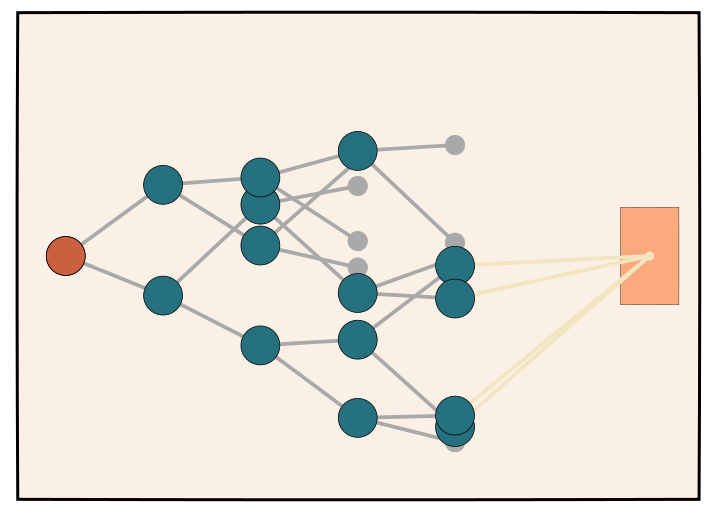
\includegraphics[width=\textwidth]{images/beamguide.png}
		\end{column}
	\end{columns}
	\blfootnote{\cite{Snell2024-dx}}
\end{frame}


\begin{frame}{Guide Variants}
	\begin{itemize}
		\item Monte Carlo Roll-outs
		\item Learned Value Function (PRM)
		\item Generative Verifier
	\end{itemize}
\end{frame}


\begin{frame}{Beam Search with Roll-Outs}
	\begin{columns}
		\begin{column}{0.5\linewidth}
			For partial $\cfz{z_{1:t-1}}$, rollout,
			$$\cfy{y}^{n} \sim p(\cdot|\cx,\cfz{z_{1:t-1}})$$

			$$\textcolor{c2}{r_{MC}}(\cfz{z_{t}}) = \frac{1}{N}\sum_{n=1}^{N} \Ver(\cy^{n})$$
		\end{column}
		\begin{column}{0.5\linewidth}
			\begin{tikzpicture}
				\foreach \i in {1,...,4}{
						\only<+>{
							\node[anchor=north west] at (0,0) {\includegraphics[width=0.9\textwidth]{images/beamroll\i}};
						}
					}
			\end{tikzpicture}
		\end{column}
	\end{columns}
	\blfootnote{\cite{Kazemnejad2024-cp}}
\end{frame}


\begin{frame}{Learned Value Function}

	\begin{columns}
		\begin{column}{0.5\linewidth}
			\begin{itemize}
				\item Rollouts are costly / require $\Ver$
				\item Learn $\textcolor{c2}{r_{\psi}}(\cfz{z_t})$ to approximate
				\item Use $\textcolor{c2}{r_{MC}}$ for labels
			\end{itemize}
		\end{column}
		\begin{column}{0.5\linewidth}
			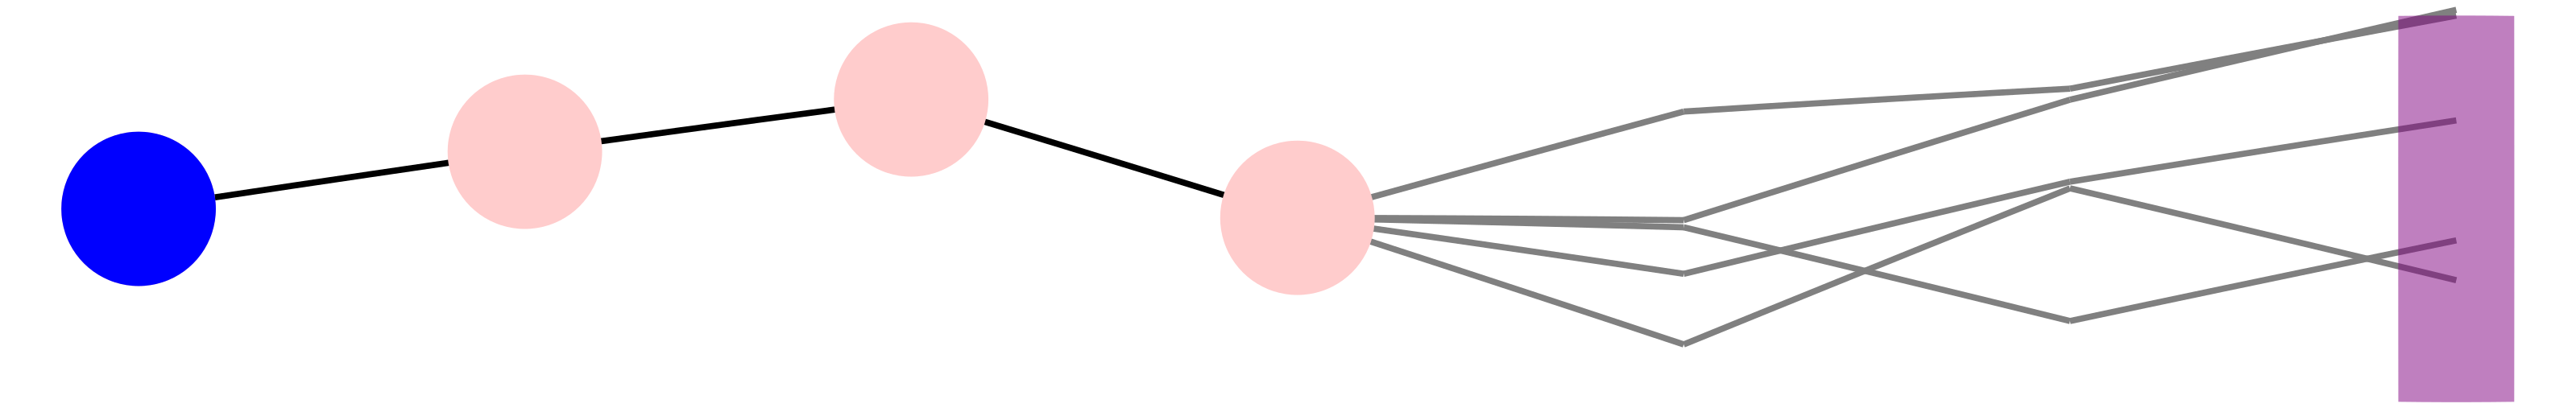
\includegraphics[width=\textwidth]{images/mcroll.png}
		\end{column}
	\end{columns}
	\blfootnote{\cite{Lightman2023-cr,Wang2023-ur}}
\end{frame}



\begin{frame}{Hybrid Value Functions}
	\begin{columns}
		\begin{column}{0.5\linewidth}
			\begin{itemize}
				\item Combine $\textcolor{c2}{r_{MC}}$ and $\textcolor{c2}{r_{\psi}}$
				\item $$\textcolor{c2}{r_{Inter}}(\cfz{z_t}) = (1-\alpha)\textcolor{c2}{r_{MC}}(\cfz{z_t}) + \alpha\textcolor{c2}{r_{\psi}}(\cfz{z_t})$$
			\end{itemize}
		\end{column}
	\end{columns}
\end{frame}


\begin{frame}{Variants}
	\begin{itemize}
		\item Search Heuristic
		\item Value Function
		\item PRM; Process Reward Model \cite{Uesato2022-aw,Lightman2023-cr}
		\item PAV; Process Advantage Verifier \cite{Setlur2024-ax}
	\end{itemize}
\end{frame}


\begin{frame}{Test-time Guides Outperform Self-consistency}
	% I think this is a nice empirical figure to show that learned rewards improve the test-time
	% performance over self-consistency.
	\blfootnote{\cite{Wang2023-ur}}
	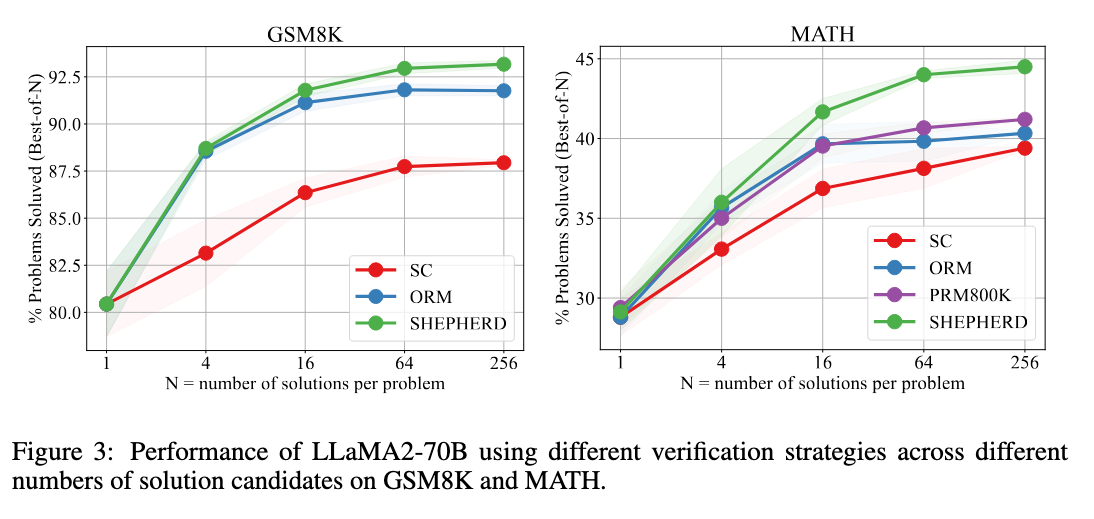
\includegraphics[width=\textwidth]{images/math_shepherd_figure_3.png}
\end{frame}


\begin{frame}{Is this o1?}
	\begin{itemize}
		\item[$\boldsymbol{\checkmark}$] RS needs to be more efficient.
		\item[$\boldsymbol{\checkmark}$] Learned rewards are effective
	\end{itemize}
	\begin{itemize}
		\item[\textcolor{red}{$\boldsymbol{\times}$}] o1 is a single test-time model
		\item[\textcolor{red}{$\boldsymbol{\times}$}] Not clear if this is enough for planning.
	\end{itemize}
\end{frame}

\begin{frame}{Training Versus Test}
	\begin{columns}
		\begin{column}{0.5\linewidth}
			\begin{itemize}
				\item Learned value could be used at test-time
				\item Alternative can be trained into LLM
				\item \textit{Generative Verifier} \cite{Zhang2024-sa}
			\end{itemize}
		\end{column}
		\begin{column}{0.5\linewidth}

			\begin{tcolorbox}[colback=white,colframe=black,boxrule=0.5pt]
				\begin{quote}

					Let’s analyze each option.
					\vspace{0.3cm}

					Option A: “because appetite regulation is a field of staggering complexity.”
					\vspace{0.3cm}

					Is that a good explanation? Hmm.
					\vspace{0.3cm}
				\end{quote}
			\end{tcolorbox}

		\end{column}
	\end{columns}
\end{frame}


\subsection{AlphaZero}
\begin{frame}{The Suspects}
	\begin{itemize}
		\item Guess + Check
		\item Guided Search
		\item \structure{AlphaZero}
		\item Learning to Correct
	\end{itemize}
\end{frame}

\begin{frame}{Reminder: AlphaZero}
	\centering
	\begin{columns}
		\begin{column}{0.6\textwidth}
			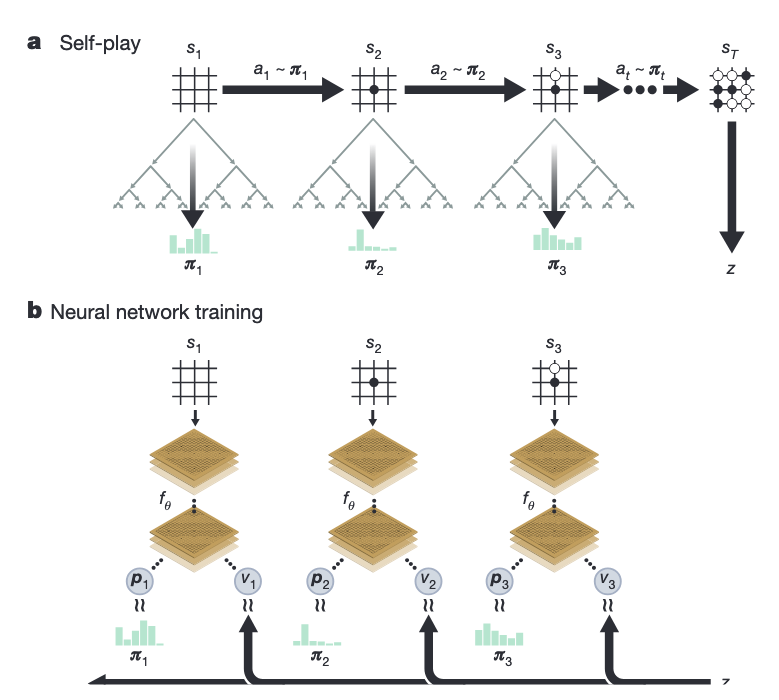
\includegraphics[height=0.8\textheight]{images/alphazero_figure_one.png}
		\end{column}
		\begin{column}{0.4\textwidth}
			\begin{itemize}
				\item Canonical example of self-learning
				\item Scaling model without data
			\end{itemize}
		\end{column}
	\end{columns}
	\blfootnote{\cite{Silver2017-bn}}
\end{frame}

\begin{frame}{Suspect 3: AlphaZero}
	\begin{itemize}
		\item 1) Self-play using guided-search with exploration
		\item 2) Label final outcomes of self-play games
		\item 3) Train guide and generator
	\end{itemize}
\end{frame}

\begin{frame}{Framework: Expert Iteration}
	% VSTaR is almost the LM equivalent of AlphaZero in the framing,
	% except that AlphaZero learns a PRM (value function) and V-STaR learns an ORM.
	% Plus AlphaZero uses its PRM during search, which V-STaR can't do.
	%
	% I wrote this with the reward model involved, but technically expert iteration doesn't
	% require that. At that point I think it reduces to Rejection Sampling EM though.
	\begin{itemize}
		\item Iterative algorithm combining learned model + expert search with a verifier.
		\item Generate samples using $p(\cy,\cz|\cx)$, reward model $r(\cz_t)$, and search algorithm (e.g. beam search)
		\item Label samples using $\Ver_x(\cy)$
		\item Train $p(\cy,\cz|\cx)$, $r(\cz_t)$ on the labeled samples, and repeat
	\end{itemize}
	\blfootnote{\cite{Anthony2017-dm}}

\end{frame}

\begin{frame}{Review: MCTS}
	% Not sure if there's a way to formalize this for language models, since
	% we're unlikely to get the same z twice (i.e. end up in the same state/action pair).
	% That means the state visit counts in the usual UCB formulation don't work.
	% The exploration in previous methods here has come from sampling or
	% maintaining multiple candidates, rather than tracking UCB statistics.
	\begin{center}
		\foreach \i in {10,...,30}{
				\only<\i>{\includegraphics[width=0.9\textwidth]{images/mcts0\i}}
			}
	\end{center}
	\blfootnote{\cite{Kocsis2006-er}}
\end{frame}


\begin{frame}{UCB for Language}
	\begin{itemize}
		\item \textbf{Selection}: Walk down tree to leaf $\cfz{z_{t-1}}$
		\item \textbf{Expand}: Sample $~5$ next steps $\cfz{z_t}$, pick one at random
		\item \textbf{Rollouts}: Sample steps $\cfz{z_{t+1}} \ldots \cfz{z_T}$
		\item \textbf{Backprop}: Update nodes counts $N(z_{1:t})$ based on results
	\end{itemize}
	\blfootnote{\cite{Hubert2021-ju,Feng2023-sz}}
\end{frame}


\begin{frame}{Compared with Guided Search}
	\begin{itemize}
		\item MCTS-UCB explores states
		      $$ \sqrt{\frac{\ln N(\cfz{z_{1:t-1}})}{N(\cfz{z_{1:t})}}} $$
		\item Less strict search process
	\end{itemize}
\end{frame}

\begin{frame}{Empirical Results}
	% figure from appendix of the VSTaR paper
	% VSTaR is sort of a weird variation of expert iteration. The learned model is
	% both the generator and the verifier, but only the generator influences the
	% expert search (since it determines what the samples are at the next iteration that the verifier labels).
	% I think it still falls within expert iteration, though, just with an expert policy
	% that's independent of the reward model.
	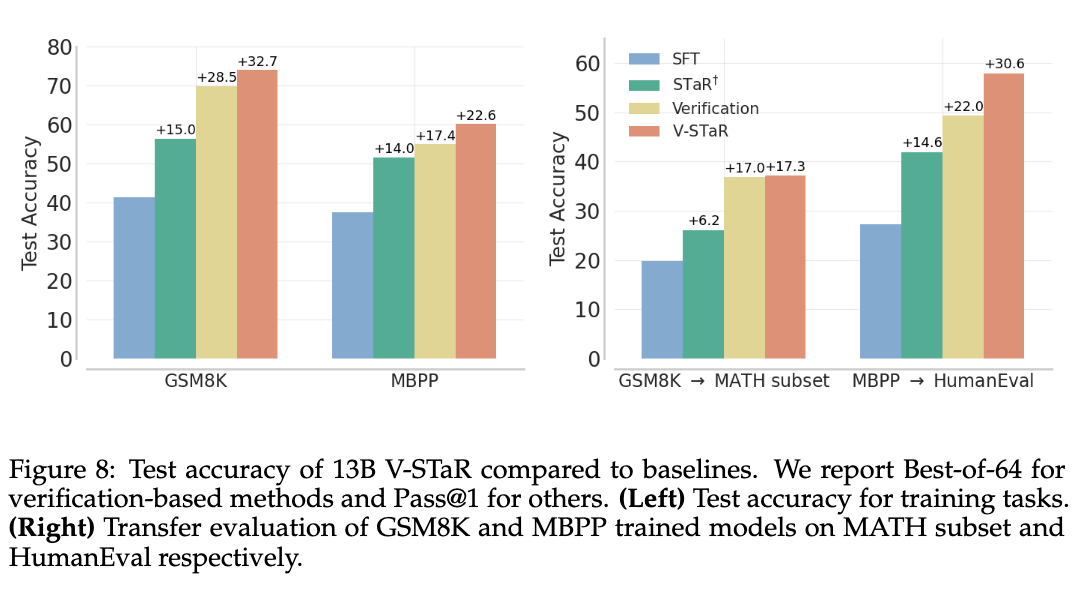
\includegraphics[width=\textwidth]{images/vstar_figure_8.png}
	\blfootnote{\cite{hosseini2024vstar}}
\end{frame}


\begin{frame}{Is this o1?}
	\begin{columns}
		\begin{column}{0.5\linewidth}
			\begin{itemize}
				\item[$\boldsymbol{\checkmark}$] Major demonstrated RL result
				\item[$\boldsymbol{\checkmark}$] Scales to more train-time search
			\end{itemize}
		\end{column}
		\begin{column}{0.5\linewidth}
			\begin{itemize}
				\item[\textcolor{red}{$\boldsymbol{\times}$}] Costly to maintain open states
				\item[\textcolor{red}{$\boldsymbol{\times}$}] More complex algorithmically
			\end{itemize}
		\end{column}
	\end{columns}
\end{frame}

\subsection{Learning to Correct}

\begin{frame}{The Suspects}
	\begin{itemize}
		\item Guess + Check
		\item Guided Search
		\item AlphaZero
		\item \structure{Learning to Correct}
	\end{itemize}
\end{frame}

\begin{frame}{What does exploration look like?}
	\begin{itemize}
		\item Game Playing - Explore alternative moves.
		\item Language - Nearly infinite "moves"
		\item Exploration to learn strategies
	\end{itemize}

\end{frame}

\begin{frame}{Suspect 4: Learning to Correct}
	\begin{itemize}
		\item 1) Sample $N$ Successful CoTs
		\item 2) Edit to inject incorrect expansions before
		      correct ones.
		\item 3) Train on correcting trajectories
	\end{itemize}
\end{frame}


\begin{frame}{Self-Correction}
	\begin{itemize}
		\item Argument: Training on $\cx, \cfz{z^*_1}, \cy$ is too easy.
		\item Train instead on $\cx, \cfz{z'}, \cfz{z^*_1}, \cy$
		\item Model should learn to self-correct
	\end{itemize}
	\blfootnote{\cite{Gandhi2024-vs}}
\end{frame}

\begin{frame}{Score}
	\begin{itemize}
		\item Positive rewards
	\end{itemize}
\end{frame}


\begin{frame}{Challenge: Collapse}
	\begin{itemize}
		\item Model may learn to just ignore negative
		\item
		\item
	\end{itemize}
\end{frame}


\begin{frame}{Generalized: Stream of Search}
	\begin{itemize}
		\item Find $\cfz{z^*_{1:T}}$ as optimal length CoT
		\item Find $\cfz{z'_{1:T'}}$ with $T' > T$ through backtracking tree search
		\item Train model on $\cfz{z'_{1:T'}}$
	\end{itemize}
	\blfootnote{\cite{Gandhi2024-vs}}
\end{frame}

\begin{frame}{From Tree to Stream}
	\begin{columns}
		\begin{column}{0.5\linewidth}
			\begin{itemize}
				\item Tree search explores multiple paths
				\item Stream presents a linear sequence
				\item Allows model to learn from mistakes
			\end{itemize}
		\end{column}
		\begin{column}{0.5\linewidth}
			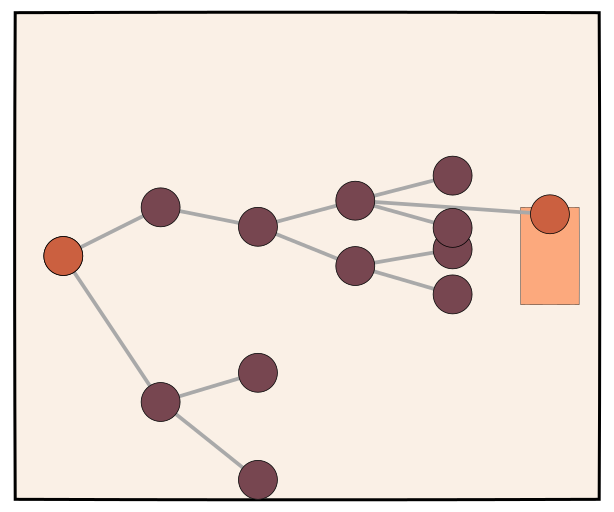
\includegraphics[width=\textwidth]{images/search}
			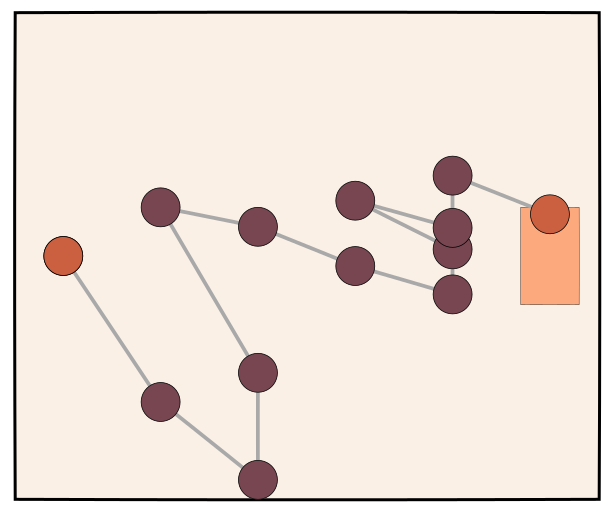
\includegraphics[width=\textwidth]{images/search2}
		\end{column}
	\end{columns}
	\blfootnote{\cite{Gandhi2024-vs}}
\end{frame}

\begin{frame}{Empirical Results}
	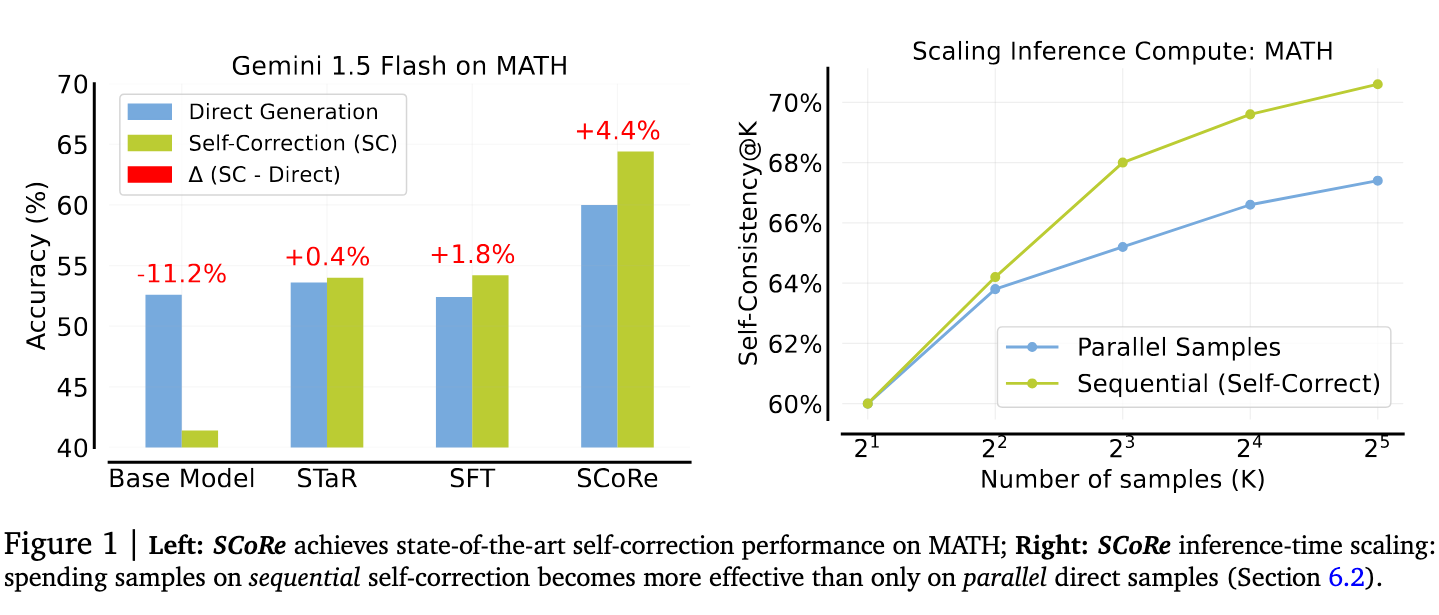
\includegraphics[width=\textwidth]{images/score_figure_1.png}
\end{frame}
\begin{frame}{Empirical Results}
	% This one is more detailed than figure 1, but we can also cut it out if
	% it makes more sense to just have the one figure with MATH performance and compute scaling
	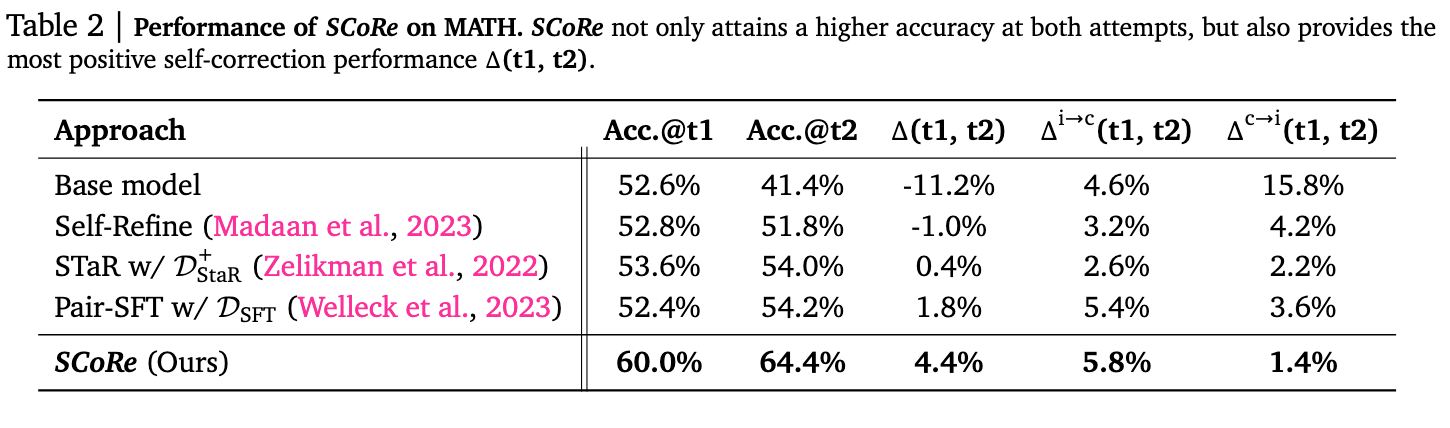
\includegraphics[width=\textwidth]{images/score_table_2.png}
\end{frame}

\begin{frame}{Is this o1?}
	\begin{columns}
		\begin{column}{0.5\linewidth}
			\begin{itemize}
				\item[$\boldsymbol{\checkmark}$] Learns to correct and plan
				\item[$\boldsymbol{\checkmark}$] Single test-time model
			\end{itemize}
		\end{column}
		\begin{column}{0.5\linewidth}
			\begin{itemize}
				\item[\textcolor{red}{$\boldsymbol{\times}$}] Complex training process
				\item[\textcolor{red}{$\boldsymbol{\times}$}] Limited empirical evidence
			\end{itemize}
		\end{column}
	\end{columns}
\end{frame}

\section{What do we do now?}

\begin{frame}{Outline}
	\tableofcontents[hideallsubsections, currentsection]
\end{frame}

\begin{frame}{Does it need to be the same?}
	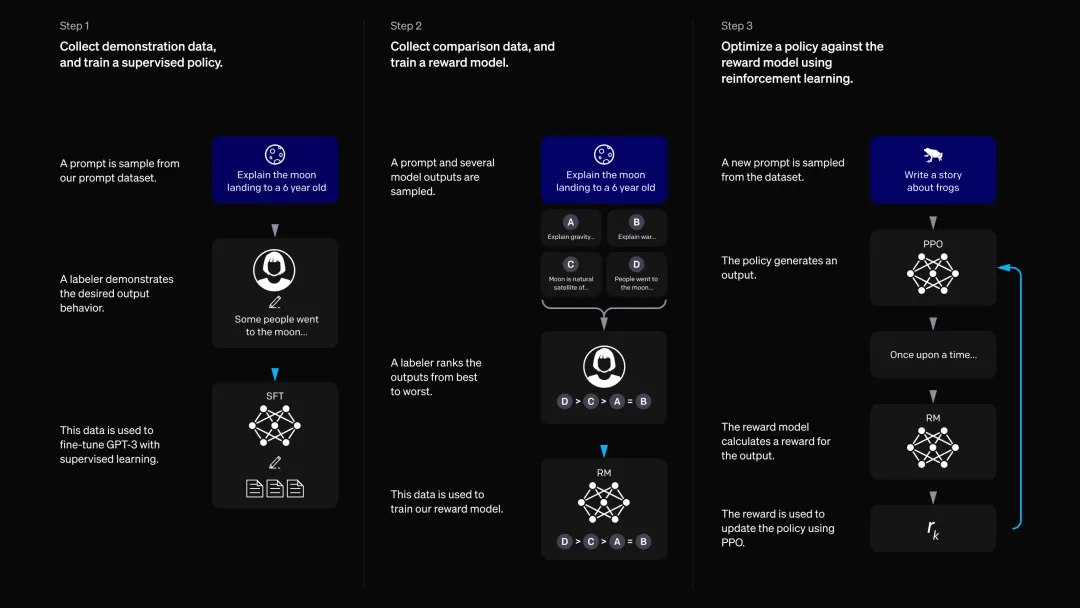
\includegraphics[width=\textwidth]{images/align}
	\blfootnote{\cite{Ouyang2022-ut}}
\end{frame}

\begin{frame}{Open-Source Models}
	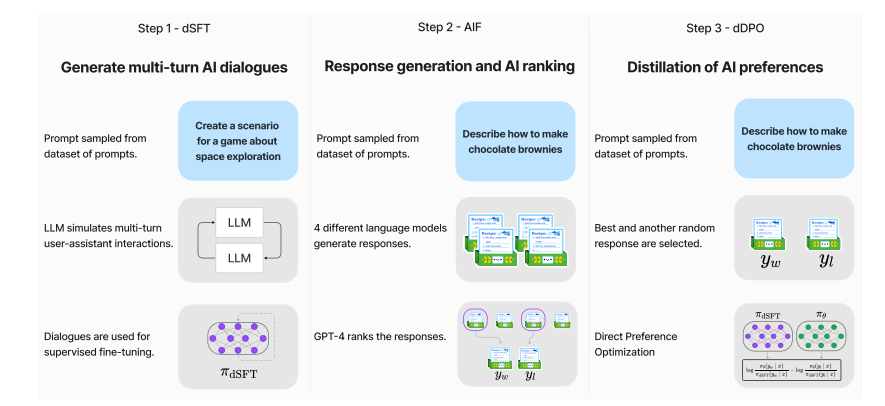
\includegraphics[width=\textwidth]{images/zephyr.png}
	\blfootnote{\cite{Tunstall2023-kv}}
\end{frame}

\begin{frame}{Replication}

	\begin{itemize}
		\item Once result is established there might be an easier path
		\item
	\end{itemize}

	\blfootnote{\cite{Putta2024-yy}}
\end{frame}

\begin{frame}[allowframebreaks]{Reference}
	\begin{small}
		\bibliographystyle{apalike}
		\bibliography{../o1.bib,../o1.extra.bib}
	\end{small}
\end{frame}

\end{document}
